% Search for all the places that say "PUT SOMETHING HERE".

\documentclass[11pt]{article}
\usepackage{amsmath,textcomp,amssymb,graphicx,enumerate,hyperref,enumitem,mathtools,tikz-qtree,listings,chemformula,bm,graphicx,grffile,gensymb,physics,amssymb,datetime,siunitx,multicol,pgfplots}
\graphicspath{{/Users/jonathansun5/Documents/Fall 2017/MCB 166/Homeworks/HW 5/Screen Shot 2017-11-12 at 11.34.36 PM.png} {/Users/jonathansun5/Documents/Fall 2017/MCB 166/Homeworks/HW 5/Screen Shot 2017-11-12 at 11.40.17 PM.png} {/Users/jonathansun5/Documents/Fall 2017/MCB 166/Homeworks/HW 5/Screen Shot 2017-11-13 at 11.42.43 PM.png} {/Users/jonathansun5/Documents/Fall 2017/MCB 166/Homeworks/HW 5/Screen Shot 2017-11-14 at 11.01.42 AM.png}}
\pgfplotsset{compat=1.14}
\makeatletter
\newcommand{\leqnos}{\tagsleft@true\let\veqno\@@leqno}
\newcommand{\reqnos}{\tagsleft@false\let\veqno\@@eqno}
\reqnos
\makeatother

\def\Name{Jonathan Sun}  % Your name
\def\SID{25020651}  % Your student ID number
\def\Homework{5} % Number of Homework
\def\Session{Fall 2017}


\title{MCB166 --- \Session --- Problem Set \Homework}
\author{\Name, SID \SID}
\markboth{MCB166 --- \Session --- Problem Set \Homework --- \Name}{MCB166 --- \Session --- Problem Set \Homework --- \Name}
\pagestyle{myheadings}
\newdate{date}{14}{11}{2017}
\date{\displaydate{date}}

\def\endproofmark{$\Box$}
\newenvironment{proof}{\par{\bf Proof:}}{\endproofmark\smallskip}

\usepackage[margin=1in]{geometry}



\begin{document}
\maketitle

\newpage
\begin{enumerate}[label=\arabic*.]
\item
The coxal muscle receptor of the crab is innervated by two large nerve fibers (Roberts \& Bush, $1971$). One of them, the T-fiber, is about $60 \mu \text{m}$ in diameter and $3 \text{mm}$ long. Two microelectrodes were inserted close together into the middle region of the fiber, one to pass stimulating currents and one for recording. Fig. A shows some of the results of one experiment. You may assume that the space constant is long relative to the fiber.
\begin{enumerate}[label=(\alph*)]
\item
Plot the results as a voltage-current graph.
\begin{center}
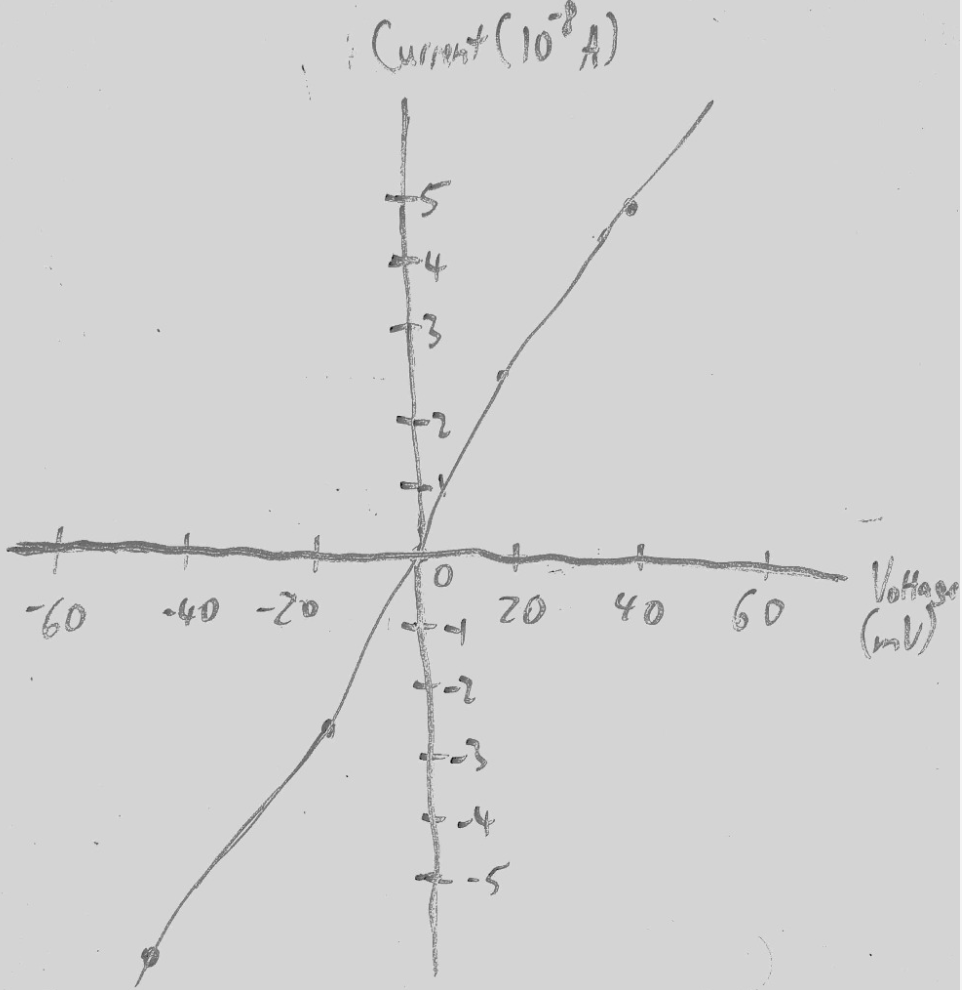
\includegraphics[width=0.75\textwidth]{/Users/jonathansun5/Documents/Fall 2017/MCB 166/Homeworks/HW 5/Screen Shot 2017-11-13 at 11.42.43 PM.png}
\end{center}



\item
What is the input resistance of the fiber?
\vspace*{1\baselineskip}
\\
Since the plot basically gives a straight line, I will use the points $\left(0 \text{mV}, 0 \text{A}\right)$ and $\left(20 \text{mV}, 2.5 \times 10^{-8} \text{A}\right)$ to calculate the resistance:
\begin{align*}
R_{in} &= \frac{\Delta V} {\Delta I} \\
&= \frac{20 \text{mV} - 0 \text{mV}} {2.5 \times 10^{-8} \text{A} - 0 \text{A}} \\
&= 800000 \Omega \\
&= 800 \text{k}\Omega
\end{align*}
Therefore, the input resistance of the fiber is about $800 \text{k}\Omega$.



\item
Give an estimate of the specific membrane resistance.
\vspace*{1\baselineskip}
\\
Since the input resistance is about $800000 \Omega$ and we were given that the T-fiber's diameter is about $60 \mu \text{m} = 6 \times 10^{-5} \text{m}$ and its length is $3 \text{mm} = 0.003 \text{m}$:
\begin{align*}
r_m &= R_{in} \times A \\
&= 800000 \Omega \times \left(\pi d l\right) \\
&= 800000 \Omega \times \left(\pi \times 6 \times 10^{-5} \text{m} \times 0.003 \text{m}\right) \\
&\approx 800000 \Omega \times 5.655 \times 10^{-7} \text{m}^2 \\
&\approx 0.452 \Omega \text{m}^2
\end{align*}
Therefore, the specific membrane resistance is about $0.452 \Omega \text{m}^2$.



\item
If the assumption is untrue and the space constant is comparable to or shorter than the fiber, would the specific resistance of the membrane be higher or lower? Give brief reasons.
\vspace*{1\baselineskip}
\\
If the assumption was false and the space constant is comparable to or shorter than the fiber, then the area itself would have been smaller. Since the specific membrane resistance is proportional to the area given the input resistance, then a smaller area would result in a smaller specific membrane resistance.
\end{enumerate}



\newpage
\item
A neuromuscular junction is stimulated $25$ times. The amplitudes of the EPPs for each of the $25$ trials are (in mV): $0.3$, $0$, $0.5$, $0.7$, $0$, $1.1$, $1.5$, $0$, $1.1$, $0.9$, $0$, $0$, $1.3$, $1.1$, $0.5$, $0.5$, $0.7$, $0$, $0.7$, $1.1$, $0.5$, $0.5$, $0$, $0.9$, $1.3$.
\begin{enumerate}[label=(\alph*)]
\item
Plot an amplitude histogram of the responses using a bin width of $0.2 \text{mV}$.
\\
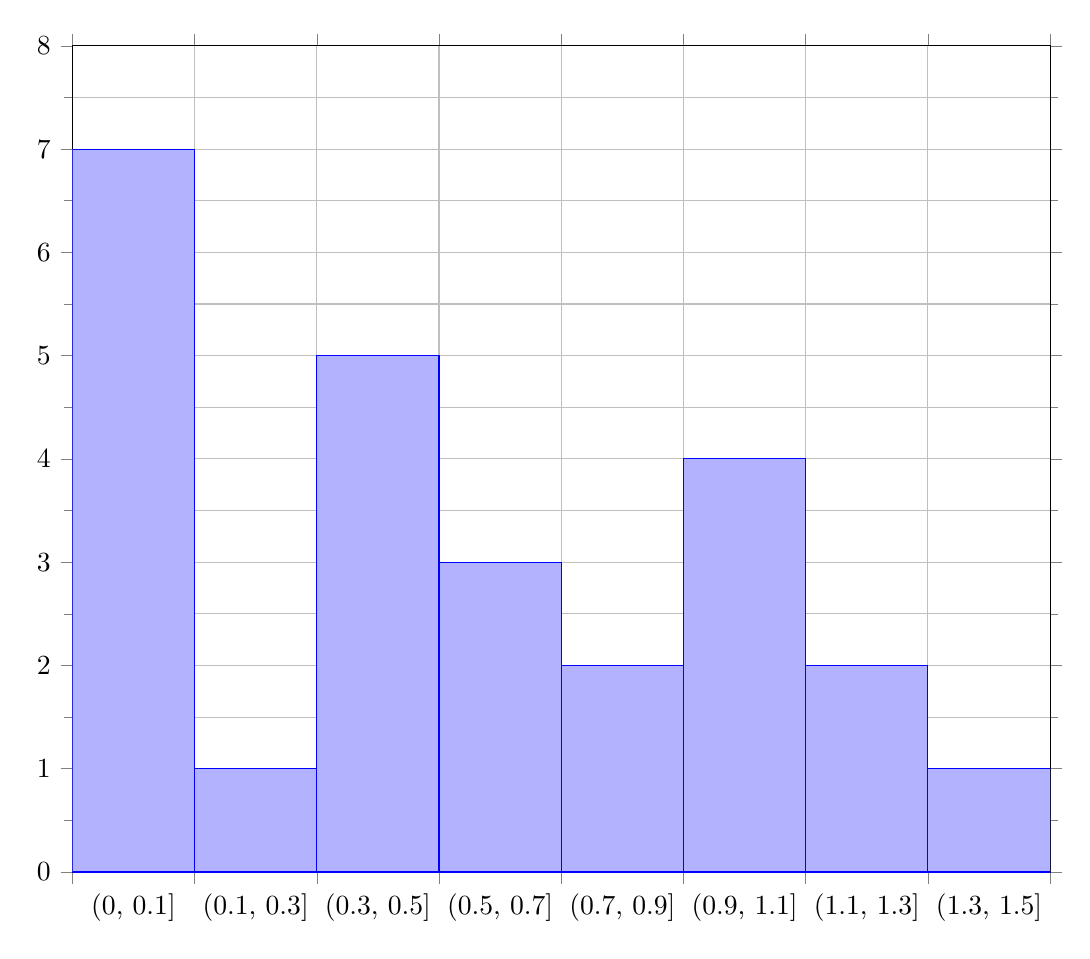
\begin{tikzpicture}
\begin{axis}[
	xticklabels={\text{(0, 0.1]}, \text{(0.1, 0.3]}, \text{(0.3, 0.5]}, \text{(0.5, 0.7]}, \text{(0.7, 0.9]}, \text{(0.9, 1.1]}, \text{(1.1, 1.3]}, \text{(1.3, 1.5]}, \text{(1.5, 1.7]}},
    xtick=data,
	ybar interval,
    ymin=0, ymax=8,
    xmin=0, xmax=1.6,
    minor y tick num=1,
    yminorgrids=false,
    grid=both,
    tick align=outside,
    width=14cm,
    ]
	\addplot+[ybar interval, mark=none] plot coordinates {
		(0.0, 7)
		(0.2, 1)
		(0.4, 5)
		(0.6, 3)
		(0.8, 2)
		(1.0, 4)
		(1.2, 2)
		(1.4, 1)
		(1.6, 0)
	};
\end{axis}
\end{tikzpicture}



\item
In other experiments you determined that the mean amplitude of the mEPP was $0.5 \text{mV}$. Calculate $m$ by at least two methods, assuming Poisson statistics for the release process.
\vspace*{1\baselineskip}
\\
Using the Direct Method:
\begin{align*}
m &= \frac{\bar{V}} {\bar{q}} \\
&= \frac{\frac{0.3 + 0 + 0.5 + 0.7 + 0 + 1.1 + 1.5 + 0 + 1.1 + 0.9 + 0 + 0 + 1.3 + 1.1 + 0.5 + 0.5 + 0.7 + 0 + 0.7 + 1.1 + 0.5 + 0.5 + 0 + 0.9 + 1.3} {25}} {0.5} \\
&= 1.216
\end{align*}
Using the Failure Method:
\begin{align*}
m &= \ln{\frac{N} {N_0}} \\
&= \ln{\frac{25} {7}} \\
&\approx 1.273
\end{align*}



\item
Given your value for $m$, how many times would you predict that $3$ quanta would be released in an experiment in which the nerve was stimulated $200$ times?
\vspace*{1\baselineskip}
\\
From the Direct Method and Failure Method above, I got $m = 1.216$ and $m \approx 1.273$. So, I will use the average between the two to get $m = 1.2445$ and use this in my calculation below:
\begin{align*}
N_3 &= \frac{m^3 e^{-m}} {6} \times N \\
&= \frac{(1.2445)^3 e^{-1.2445}} {6} \times 200 \\
&\approx 18.509
\end{align*}
Since $N_3 \approx 18.509$, I would predict $18$ times.
\end{enumerate}



\newpage
\item
Reproduced below is part of figure $12.16$. It depicts different aspects of synaptic transmission as studied at the squid giant synapse. Label and describe all parts of the figure.
\begin{center}
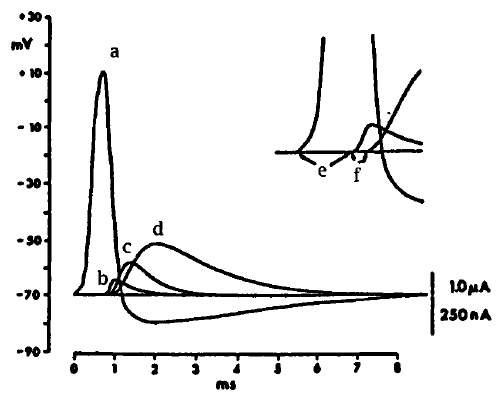
\includegraphics[width=0.75\textwidth]{/Users/jonathansun5/Documents/Fall 2017/MCB 166/Homeworks/HW 5/Screen Shot 2017-11-12 at 11.34.36 PM.png}
\end{center}
Part (a) of the graph shows the action potential, part (b) shows the presynaptic \ch{Ca^{2+}} current, part (c) shows the postsynaptic current (EPSC), and part (d) shows the postsynaptic potential (EPSP). Part (e) of the blowup figure shows the delay between the action potential and the onset of the \ch{Ca^{2+}} current. Part (f) of the blowup figure shows the delay between the \ch{Ca^{2+}} current and the onset of the postsynaptic current of part (c).



\newpage
\item
We are going to compare two models for \ch{Na} and \ch{K} currents in parallel. In the first model (A) the conductors are \underline{constant-field rectifiers}. In the second model (B), they are linear conductors with Nernst-potential barriers.
\begin{center}
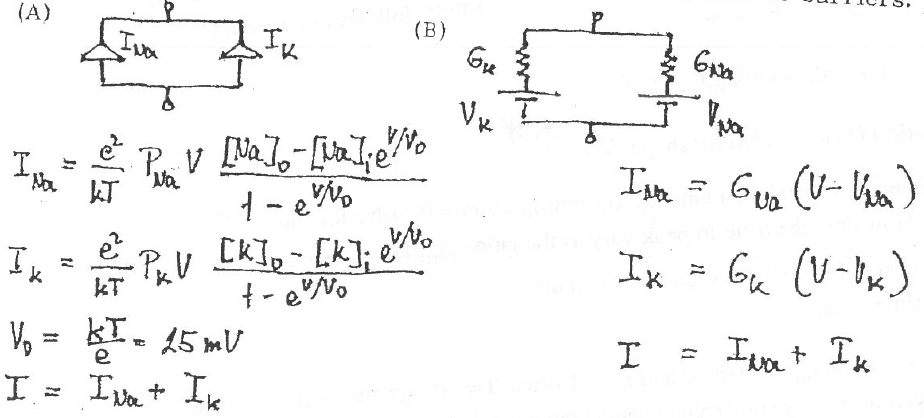
\includegraphics[width=0.75\textwidth]{/Users/jonathansun5/Documents/Fall 2017/MCB 166/Homeworks/HW 5/Screen Shot 2017-11-12 at 11.40.17 PM.png}
\end{center}
\begin{enumerate}[label=(\alph*)]
\item
For each model, write the expression for the resting potential, i.e. the potential at which $I_{\ch{Na}} + I_{\ch{K}} = 0$.
\vspace*{1\baselineskip}
\\
At the resting membrane potential, the total current is $0$ so for Model A:
\begin{align*}
I_{\ch{Na}} + I_{\ch{K}} = 0
\end{align*}
\begin{align*}
\frac{e^2} {kT} P_{\ch{Na}} V \frac{[\ch{Na}]_0 - [\ch{Na}]_i e^{\frac{V} {\frac{kT} {e}}}} {1 - e^{\frac{V} {\frac{kT} {e}}}} + \frac{e^2} {kT} P_{\ch{K}} V \frac{[\ch{K}]_0 - [\ch{K}]_i e^{\frac{V} {\frac{kT} {e}}}} {1 - e^{\frac{V} {\frac{kT} {e}}}} = 0
\end{align*}
\begin{align*}
P_{\ch{Na}} \left([\ch{Na}]_0 - [\ch{Na}]_i e^{\frac{V} {\frac{kT} {e}}}\right) + P_{\ch{K}} \left([\ch{K}]_0 - [\ch{K}]_i e^{\frac{V} {\frac{kT} {e}}}\right) = 0
\end{align*}
\begin{align*}
\left(P_{\ch{Na}} [\ch{Na}]_0 + P_{\ch{K}} [\ch{K}]_0\right) - \left(P_{\ch{Na}} [\ch{Na}]_i + P_{\ch{K}} [\ch{K}]_i\right) e^{\frac{V} {\frac{kT} {e}}} = 0
\end{align*}
\begin{align*}
e^{\frac{V} {\frac{kT} {e}}} = \frac{P_{\ch{Na}} [\ch{Na}]_0 + P_{\ch{K}} [\ch{K}]_0} {P_{\ch{Na}} [\ch{Na}]_i + P_{\ch{K}} [\ch{K}]_i}
\end{align*}
\begin{align*}
\frac{V} {\frac{kT} {e}} = \ln{\frac{P_{\ch{Na}} [\ch{Na}]_0 + P_{\ch{K}} [\ch{K}]_0} {P_{\ch{Na}} [\ch{Na}]_i + P_{\ch{K}} [\ch{K}]_i}}
\end{align*}
\begin{align*}
V = \frac{kT} {e} \ln{\frac{P_{\ch{Na}} [\ch{Na}]_0 + P_{\ch{K}} [\ch{K}]_0} {P_{\ch{Na}} [\ch{Na}]_i + P_{\ch{K}} [\ch{K}]_i}}
\end{align*}
For Model B:
\begin{align*}
I_{\ch{Na}} + I_{\ch{K}} = 0
\end{align*}
\begin{align*}
G_{\ch{Na}}\left(V - V_{\ch{Na}}\right) + G_{\ch{K}}\left(V - V_{\ch{K}}\right) = 0
\end{align*}
\begin{align*}
G_{\ch{Na}} V - G_{\ch{Na}} V_{\ch{Na}} + G_{\ch{K}} V - G_{\ch{K}} V_{\ch{K}} = 0
\end{align*}
\begin{align*}
G_{\ch{Na}} V + G_{\ch{K}} V = G_{\ch{Na}} V_{\ch{Na}} + G_{\ch{K}} V_{\ch{K}}
\end{align*}
\begin{align*}
V = \frac{G_{\ch{Na}} V_{\ch{Na}} + G_{\ch{K}} V_{\ch{K}}} {G_{\ch{Na}} + G_{\ch{K}}}
\end{align*}



\item
For model (A), show that as $V \rightarrow \infty$ or $V \rightarrow -\infty$ (i.e. become very large), $I(V)$ becomes linear but with different slopes. The ratio these slopes is called the rectification ratio. Write the resting potential for rectification ratio $= 1$.
\vspace*{1\baselineskip}
\\
The current for Model A is represented as:
\begin{align*}
I(V) &= \frac{e^2} {kT} P_{\ch{Na}} V \frac{[\ch{Na}]_0 - [\ch{Na}]_i e^{\frac{V} {\frac{kT} {e}}}} {1 - e^{\frac{V} {\frac{kT} {e}}}} + \frac{e^2} {kT} P_{\ch{K}} V \frac{[\ch{K}]_0 - [\ch{K}]_i e^{\frac{V} {\frac{kT} {e}}}} {1 - e^{\frac{V} {\frac{kT} {e}}}} \\
&= \frac{e^2} {kT} V \left(P_{\ch{Na}} \frac{[\ch{Na}]_0 - [\ch{Na}]_i e^{\frac{V} {\frac{kT} {e}}}} {1 - e^{\frac{V} {\frac{kT} {e}}}} + P_{\ch{K}} \frac{[\ch{K}]_0 - [\ch{K}]_i e^{\frac{V} {\frac{kT} {e}}}} {1 - e^{\frac{V} {\frac{kT} {e}}}}\right)
\end{align*}
Basically, we need to show that $\left(P_{\ch{Na}} \frac{[\ch{Na}]_0 - [\ch{Na}]_i e^{\frac{V} {\frac{kT} {e}}}} {1 - e^{\frac{V} {\frac{kT} {e}}}} + \frac{e^2} {kT} P_{\ch{K}} \frac{[\ch{K}]_0 - [\ch{K}]_i e^{\frac{V} {\frac{kT} {e}}}} {1 - e^{\frac{V} {\frac{kT} {e}}}}\right)$ is constant as $V \rightarrow \pm \infty$. \\
For $\lim_{V \rightarrow -\infty} I(V)$:
\begin{align*}
\lim_{V \rightarrow -\infty} I(V) &= \frac{e^2} {kT} V \left(P_{\ch{Na}} \frac{[\ch{Na}]_0 - [\ch{Na}]_i e^{\frac{V} {\frac{kT} {e}}}} {1 - e^{\frac{V} {\frac{kT} {e}}}} + P_{\ch{K}} \frac{[\ch{K}]_0 - [\ch{K}]_i e^{\frac{V} {\frac{kT} {e}}}} {1 - e^{\frac{V} {\frac{kT} {e}}}}\right) \\
&= \frac{e^2} {kT} V \left(P_{\ch{Na}} [\ch{Na}]_0 + P_{\ch{K}} [\ch{K}]_0\right) \\
\end{align*}
For $\lim_{V \rightarrow +\infty} I(V)$:
\begin{align*}
\lim_{V \rightarrow -\infty} I(V) &= \frac{e^2} {kT} V \left(P_{\ch{Na}} \frac{[\ch{Na}]_0 - [\ch{Na}]_i e^{\frac{V} {\frac{kT} {e}}}} {1 - e^{\frac{V} {\frac{kT} {e}}}} + P_{\ch{K}} \frac{[\ch{K}]_0 - [\ch{K}]_i e^{\frac{V} {\frac{kT} {e}}}} {1 - e^{\frac{V} {\frac{kT} {e}}}}\right) \\
&= \frac{e^2} {kT} V \left(P_{\ch{Na}} [\ch{Na}]_i + P_{\ch{K}} [\ch{K}]_i\right) \\
\end{align*}
Since I can represent $I(V)$ when $V \rightarrow -\infty$ and $V \rightarrow +\infty$ as $m_1 V$ and $m_2 V$ respectively, I can define $\frac{m_1} {m_2} = e^{\frac{V} {V_0}}$ as the rectification ratio:
\begin{align*}
m_1 = \frac{e^2} {kT} \left(P_{\ch{Na}} [\ch{Na}]_0 + P_{\ch{K}} [\ch{K}]_0\right) \\
\end{align*}
\begin{align*}
m_2 = \frac{e^2} {kT} \left(P_{\ch{Na}} [\ch{Na}]_i + P_{\ch{K}} [\ch{K}]_i\right) \\
\end{align*}
\begin{align*}
e^{\frac{V} {V_0}} = \frac{m_1} {m_2} = \frac{\frac{e^2} {kT} \left(P_{\ch{Na}} [\ch{Na}]_0 + P_{\ch{K}} [\ch{K}]_0\right)} {\frac{e^2} {kT} \left(P_{\ch{Na}} [\ch{Na}]_i + P_{\ch{K}} [\ch{K}]_i\right)} = \frac{P_{\ch{Na}} [\ch{Na}]_0 + P_{\ch{K}} [\ch{K}]_0} {P_{\ch{Na}} [\ch{Na}]_i + P_{\ch{K}} [\ch{K}]_i}
\end{align*}
Therefore, I get:
\begin{align*}
\frac{V} {V_0} = \ln{\frac{P_{\ch{Na}} [\ch{Na}]_0 + P_{\ch{K}} [\ch{K}]_0} {P_{\ch{Na}} [\ch{Na}]_i + P_{\ch{K}} [\ch{K}]_i}}
\end{align*}
\begin{align*}
V = V_0 \ln{\frac{P_{\ch{Na}} [\ch{Na}]_0 + P_{\ch{K}} [\ch{K}]_0} {P_{\ch{Na}} [\ch{Na}]_i + P_{\ch{K}} [\ch{K}]_i}}
\end{align*}
\begin{align*}
V = \frac{kT} {e} \ln{\frac{P_{\ch{Na}} [\ch{Na}]_0 + P_{\ch{K}} [\ch{K}]_0} {P_{\ch{Na}} [\ch{Na}]_i + P_{\ch{K}} [\ch{K}]_i}}
\end{align*}



\item
Show that model (B) can be written as a single element $I = \bar{G}(V - \bar{V})$. Write expressions for $\bar{G}$ and $\bar{V}$.
\begin{align*}
I &= G_{\ch{Na}}\left(V - E_{\ch{Na}}\right) + G_{\ch{K}}\left(V - E_{\ch{K}}\right) \\
&= \left(G_{\ch{Na}} + G_{\ch{K}}\right) \left(V - \frac{G_{\ch{Na}} E_{\ch{Na}} + G_{\ch{K}} E_{\ch{K}}} {G_{\ch{Na}} + G_{\ch{K}}}\right)
\end{align*}



\item
Model (B) makes no sense when any relevant ionic concentration goes to zero. This is because one of the Nernst potentials will become infinite. Explain what is wrong with the model for such a condition. Does model (A) have this trouble? If not, why not? Sketch a curve of $I_{\ch{K}}(V)$ when $[K]_0 = 0$, and describe the current.
\vspace*{1\baselineskip}
\\
In Model A, we get that $V$ is the log of sums while in Model B, we get that it is the sum of logs. Since the log of sums is not the same as the sum of logs, this is why the Model B is incorrect. Model A does not have this issue since even if there was no potassium, you can still get a valid answer with sodium only. 
\vspace*{1\baselineskip}
\\
When $[K]_0 = 0$:
\begin{align*}
I_{\ch{K}}(V) &= \frac{e^2} {kT} P_{\ch{K}} V \frac{[\ch{K}]_0 - [\ch{K}]_i e^{\frac{V} {\frac{kT} {e}}}} {1 - e^{\frac{V} {\frac{kT} {e}}}} \\
&= \frac{e^2} {kT} P_{\ch{K}} V \frac{-[\ch{K}]_i e^{\frac{V} {\frac{kT} {e}}}} {1 - e^{\frac{V} {\frac{kT} {e}}}} \\
&= \frac{e^2} {kT} [\ch{K}]_i P_{\ch{K}} \frac{V} {1 - e^{-\frac{V} {\frac{kT} {e}}}}
\end{align*}
\begin{center}
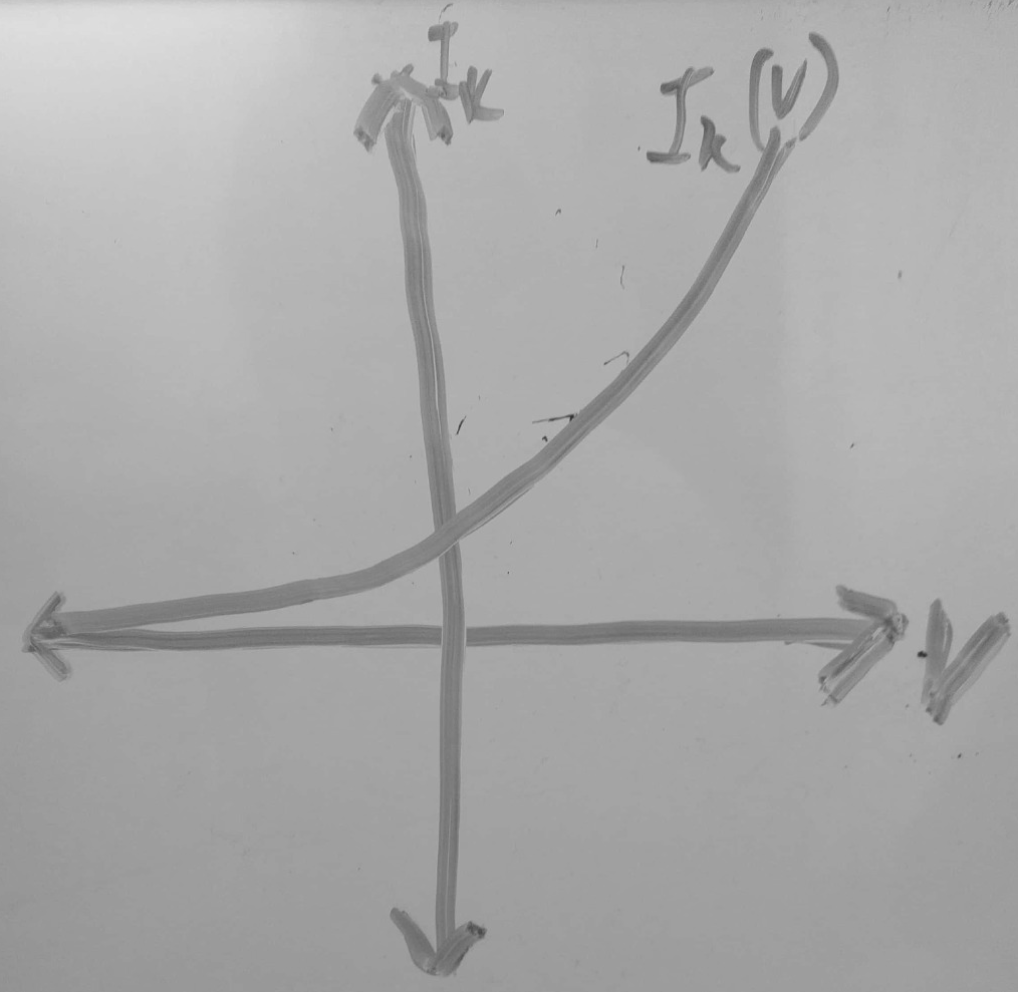
\includegraphics[width=0.75\textwidth]{/Users/jonathansun5/Documents/Fall 2017/MCB 166/Homeworks/HW 5/Screen Shot 2017-11-14 at 11.01.42 AM.png}
\end{center}
\end{enumerate}
\end{enumerate}
\end{document}
